\chapter{Výběr komponent/zařízení}

Na obrázku XXX je nákres otopné soustavy včetně  jednotlivých zařízení pro ovládání této soustavy včetně ovládání podlahové vytápění. Nyní popíši jednotlivá vybraná či navržená zařízení z nákresu.


\section{Centrální jednotka Raspberry Pi}
Pro centrální řídicí jednotku jsem vybral jednodeskový počítač Raspberry Pi model 4. Důvodem pro vybraní byla přímá podpora HA, velká uživatelská základna, která toto zařízení používá (nejen s HA, ale i s jiným softwarem), nízká a relativně vysoký výkon. V neposlední řadě na pozadí HA běží linuxová distribuce, takže ovládání je stejné jak při použití běžných desktopových verzí. Přehled specifikace zařízení je v tabulce \ref{tab:prehled-vybaveni-raspberry-pi-4-model-b}. Samotné Raspberry Pi je na obrázku \ref{fig:raspberry-pi-4-model-b}. Samozřejmě může vzniknout úvaha nad odolností tohoto zařízení např. vůči vnějšímu rušení, samotného rušení zařízení apod. Co se týče nasazení takového zařízení, většinou výrobci uvádějí že se jedná o~vývojové zařízení, které není určeno do koncového zařízení nebo případně splňují  základní certifikace ochrany. Průmyslovou certifikaci nesplňují nebo se na trhu nacházejí zařízení, které se průmyslovou aplikací chlubí (zde je nutné důkladně pročíst všechnu technickou dokumentaci), pak dále skutečně stojí za zvážení o jakou certifikaci se jedná, v jaké části průmyslu lze toto zařízení nasadit, ale i tak to může být dost velký risk. Ve většině případů je však nutné provést hardwarovou úpravu pro vysokou odolnost proti rušení, robustnost běžícího real time systému, RTC, typ paměti pro ukládání dat (typ média), životnost, technická podpora a mnohé další. V domácích podmínkách nejsou nutné všechny požadavky jako v průmyslu, nicméně je nutné minimálně hledět na ESD ochranu připojených periferií především u sběrnic, které jsou na delší vzdálenosti a způsob ukládání dat z pohledu životnosti paměťového média. Pro ESD ochranu jak samotného Raspberry Pi, tak i koncových zařízení je nutné zapojit mezi kabely sběrnice a zařízení ESD ochrany (takové ochrany jsou navrženy a popsány níže). SD kartu pro ukládání a běh samotného systému je vhodné změnit za médium s vetší životností, lze využít například domácí NAS a data ukládat do databáze, SD kartu používat pouze pro systém či USB flash disk. Případně zajistit postup s předpřipravenou zálohou pro obnovu nefunkčního systému apod. 

\begin{center}
\begin{table}[H]
\begin{tabular}{|c||c|}
\hline
\thead{Procesor} &  
\makecell{Broadcom BCM2711 \\ 
quad-core Cortex-A72 (ARM v8)
64-bit, 1,5 GHz} \\ 
\hline
\thead{RAM} & 4 GB LPDDR4 \\ 
\hline
\thead{Konektivita} & 
\makecell{2,4 GHz a 5.0 GHz IEEE 802.11b/g/n/ac \\
LAN, Bluetooth 5.0, BLE \\
Gigabit Ethernet \\
2 × USB 3.0 ports \\
2 × USB 2.0 ports} \\
\hline
\thead{GPIO} & 2 × 20 pinový header \\ 
\hline
\thead{Video a zvuk} & 
\makecell{
2 × micro HDMI porty \\
 MIPI DSI displejový port \\
 MIPI CSI kamerový port \\
čtyřpólový stereo audio a kompozitní video port} \\ 
\hline
\thead{Podpora SD karty} & Micro SD slot (pro systém a data) \\ 
\hline
\thead{Napájení} & 
\makecell{
5 V DC přes USB-C konektor (minimum 3 A) \\
5 V DC přes GPIO header \\
(minimum 3 A, bez vstupních ochran)} \\ 
\hline
\end{tabular}
\caption{Přehled vybavení Raspberry Pi 4 modelu B \cite{raspberry-pi-4-model-b-specifikace}.}
\label{tab:prehled-vybaveni-raspberry-pi-4-model-b} 
\end{table}
\end{center}


\begin{figure}[H]
    \centering
    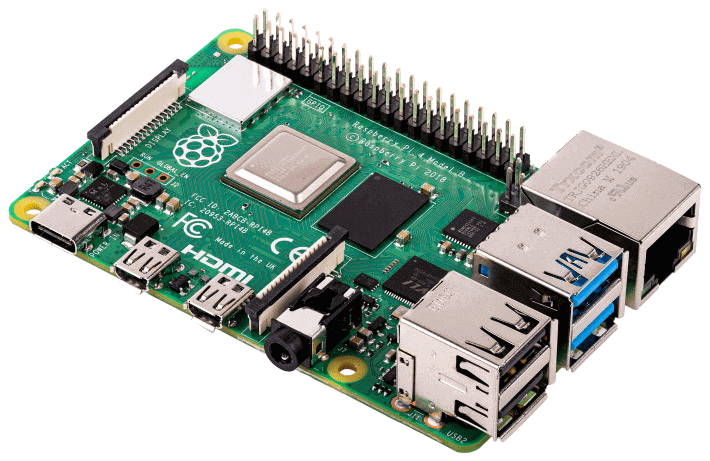
\includegraphics[width=\textwidth]{images/raspberry-pi-4-model-b.png}
    \caption{Raspberry Pi 4 model B. Upraveno z \cite{raspberry-pi-4-model-b}.}
    \label{fig:raspberry-pi-4-model-b}
\end{figure}

\section{Teplotní senzory pro krby}
\label{sec:teplotni-senzory-pro-krby}
Pro snímání teploty z kouřovodů u krbů slouží termočlánek typu K od výrobce Guenther. Teplotní rozsah je od -100 °C do 400 °C, takže je dostatečná teplotní rezerva. Průměr kovové ochranné trubičky je 4 mm s délkou 60 mm. Přívodní kabel je dlouhý 3 m se skelným opletením. Termočlánek je zobrazen na obrázku \ref{fig:termoclanek-72-21301041-k}.

\begin{figure}[H]
    \centering
    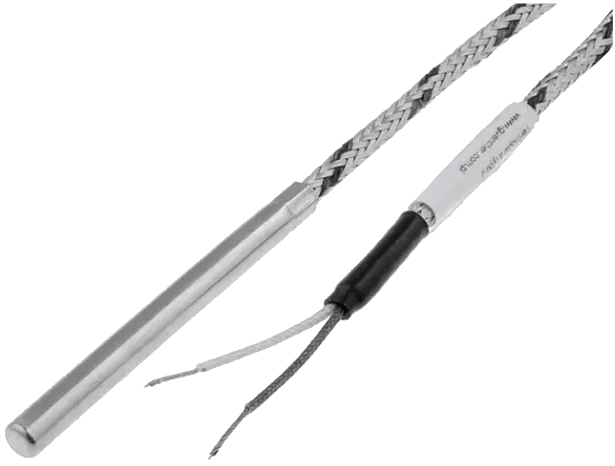
\includegraphics[width=0.5\textwidth]{images/termoclanek-72-21301041-k.png}
    \caption{Termočlánek 72-21301041 typu K \cite{termoclanek-k}.}
    \label{fig:termoclanek-72-21301041-k}
\end{figure}

\section{Teplotní senzory na 1-Wire sběrnici}
Pro snímání teplot z centrálního zásobníku otopné vody, venkovní teploty a~prostorových teplot z jednotlivých místností slouží teplotní senzor DS18B20 od výrobce Maxim. Umožňuje měřit
v teplotním rozsahu od -+55 °C do +125~°C. V rozsahu od -10 °C do +85 °C měří s přesností ±0,5 °C. Senzor umožňuje měřit teplotu s přesností 12 bitů. Pro komunikaci využívá 1-Wire sběrnici (způsob komunikace je popsán v \ref{sec:1-wire-sbernice} v části 1-Wire sběrnice). Ve svém konkrétním řešením využívám senzory v pouzdře TO-92 pro nástěnné teplotní snímače prostorové teploty, pro centrální zásobník otopné vody a~venkovní teplotu je senzor zapouzdřen do ochranného pouzdra.


\section{DPS se vstupy/výstupu pro Raspberry Pi}

\subsection{Datová část 1-Wire sběrnici}
\label{sec:datova-cast-1-wire-sbernice}
Pro zmíněnou 1-Wire sběrnici jsou realizované ESD ochrany spočívající použití Zenerovy diody a  5 $\Omega$ rezistorů, všechny součástky jsou zaintegrované v~jednom pouzdře TSOC, integrovaný obvod je od výrobce Maxim s označením DS9503. Integrovaná Zenerova dioda má nízkou kapacitu desítky pF, tím pádem nepřispívá k nadměrnému kapacitnímu zatěžování sběrnice. Omezovací rezistory slouží k omezení proudu při přepěťovém napěťovém impulzu pro ochranu Zenerovy diody (když je otevřena) před nadměrným proudem během ESD události, při běžné komunikace jsou zanedbatelné. Upínací napětí Zenerovy diody je 5,5 V při 0,9 A (průrazné napětí je přibližně 11 V) během ESD události. Dále je zde zařazena TVS dioda (ESD9L5.0ST5G) s upínacím napětí maximálně 9,8 V při 1 A, slouží jako sekundární ochrana pokud by selhala část s DS9503. 

Další možností je použití galvanického oddělení především pomocí optočlenu. Zde však nastává problém s obousměrnou poloduplexní komunikací, je potřeba zajistit komunikaci oběma směry. Optočleny vkládání zpoždění, které by podle specifikace 1-Wire sběrnice nemělo přesáhnout 1 $\mu$ s. Dále je potřeba oddělený převodník napětí či samotný zdroj pro napájení oddělených částí optočlenu a~další potřebné externí součástky. V neposlední řadě je nutné, alespoň podle výrobce Maxim použít převodník UART na 1-Wire či I$^2$C na 1-Wire sběrnici. Řešení pomocí galvanického oddělení ve výsledku zesložiťuje řešení a též prodražuje. Vzhledem k domácímu nasazení jsem se rozhodl zvolit variantu podle obrázku~\ref{fig:ochrany-1-wire}.

Vzhledem k toleranci napěťové úrovně 3,3 V pro piny u Raspberry Pi, je navržen obousměrný převodník napěťových úrovní z 3,3 V na 5~V a opačně, realizovaný pomocí MOSFET tranzistoru (BSS138P,215), pull-up rezistorů.

Na obrázku \ref{fig:ochrany-1-wire} jsou vidět dvě větve pro 1-Wire sběrnici, je to z důvodu dvou typů zařízení, teplotních čidel DS18B20 a  zesilovače s termočlánkem, které mají různé časové, popsáno více níže. Sběrnici, lze sdružit do jedné pomocí propojky P6.

\begin{figure}[H]
    \centering
    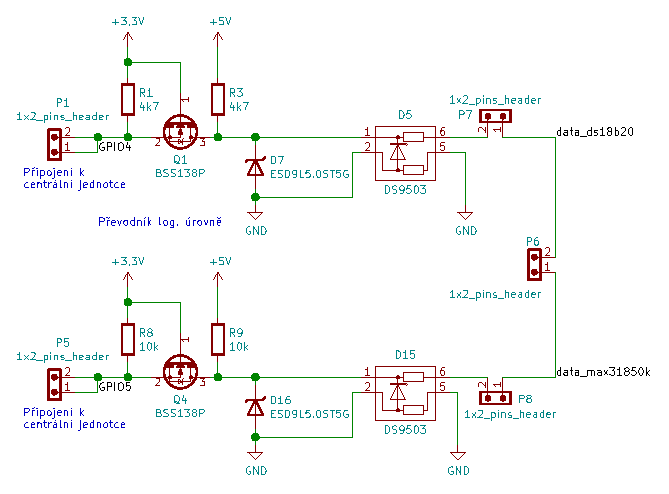
\includegraphics[width=\textwidth]{images/svg/kicad/ochrany-1-wire.eps}
    \caption[ESD ochrany pro 1-Wire sběrnici s převodním napěťových úrovní]{ESD ochrany pro 1-Wire sběrnici s převodním napěťových úrovní. Kolíková lišta P1, P5 je připojena na Raspberry Pi.}
    \label{fig:ochrany-1-wire}
\end{figure}


\subsection{Napájení 1-Wire sběrnice}
\label{napajeni-1-wire-sbernice}
Pro ochranu napájení 1-Wire sběrnice (5 V) jsou veškerá koncové teplotní senzory napájené přes elektronickou pojistku od Texas Instrumenst s označením TPS2600, obrázek \ref{fig:ochrana-napajeni-1-wire}. Která zajišťuje ochranu pro vstupní napětí, hlídá maximální hodnotu vstupního napětí do nastavené meze 5,25 V (maximální hranice je 60 V), minimální vstupní napětí do nastavené meze 4,75 V (minimální hranice je -60 V). Vstupní omezení napětí je pomocí rezistorů R5, R10, R11 a R12. Omezovací proud je nastaven na přibližně 73 mA (hodnotu lze změnit přes potenciometr R17), při jeho překročení dojde k odpojení výstupu pod dobu dokud nedojde k odstranění závady. Kondenzátor C2 nastavuje rychlost náběhu výstupního napětí. Pro indikaci chyb napájení je zde červená LED.

\begin{figure}[H]
    \centering
    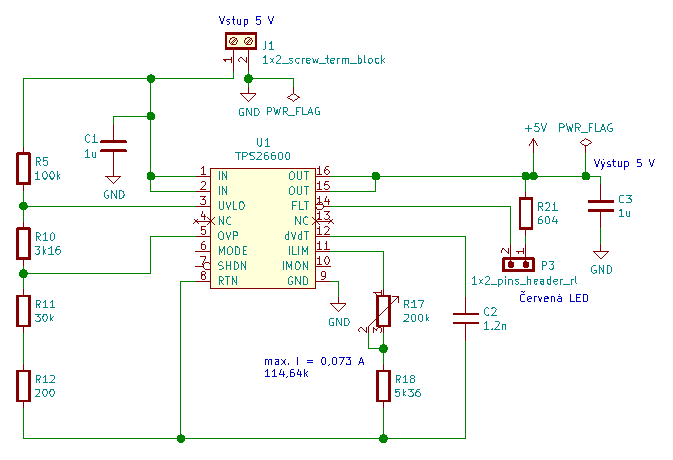
\includegraphics[width=\textwidth]{images/svg/kicad/ochrana-napajeni-1-wire.eps}
    \caption[Obvod TPS26600 pro ochranu napájení 1-Wire sběrnice.]{Obvod TPS26600 pro ochranu napájení 1-Wire sběrnice.}
    \label{fig:ochrana-napajeni-1-wire}
\end{figure}

\subsection{Ochrana pro chodbové nástěnné snímače prostorové teploty}
Obdobně jako v části \ref{sec:datova-cast-1-wire-sbernice} je stejná ochrana pro snímání log. úrovně z~chodbových nástěnných snímačů prostorové teploty.

\subsection{Ochrana napájení 3,3 V}
Přímo z Raspberry Pi je využito napětí 3,3 V pro převodník napětí, popsaný v části \ref{sec:datova-cast-1-wire-sbernice}. Zde je použita vratná pojistka polymerový PTC se spínacím proudem 100 mA, pro omezení proudu v případě poruchy, dále je zde transilová dioda pro ochranu při přepětí (s upínacím napětí max. 6,5 V (při 25 A, 10/1000~µs), průrazné napětí 3,6 V). Na obrázku \ref{fig:ochrana-napajeni-3_3-v} je zobrazena popsaná ochrana.

\begin{figure}[H]
    \centering
    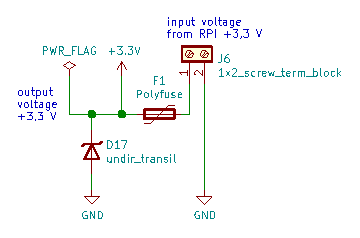
\includegraphics[width=0.6\textwidth]{images/svg/kicad/ochrana-napajeni-3_3-v.eps}
    \caption[Ochrana pro napájení 3,3 V z Raspberry Pi.]{Ochrana pro napájení 3,3 V z Raspberry Pi.}
    \label{fig:ochrana-napajeni-3_3-v}
\end{figure}

\subsection{Způsob realizace 1-Wire sběrnice}
Samotná 1-Wire sběrnice je realizovaná pomocí UTP kabelu kategorie cat5e. Na pinu číslo 4 jsou DATA, na pinu 5 je zem (GND) a na pinu 3 je napájení 5 V. Ze samotné DPS je sběrnice vyvedena pomocí konektorů RJ45, 4 konektory pro teplotní senzory DS18B20 a 4 pro termočlánky s MAX31850K.

\subsection{Realizovaná DPS ochran pro centrální jednotku Raspberry Pi}
Na obrázku \ref{fig:dps-rpi-1-wire-termostaty-ochrany-spodek} a \ref{fig:dps-rpi-1-wire-termostaty-ochrany-vrsek} je realizovaná deska plošných spojů pro vstupy/výstupů pro centrální jednotku Raspberry Pi. Deska byla vlastnoručně navržena, vyrobena a osazena. Je aplikován ochranný lak, na vrchní propojky byl též aplikován ochranný lak a následně zakryty tavnou plastovou hmotou.

\begin{figure}[H]
    \centering
    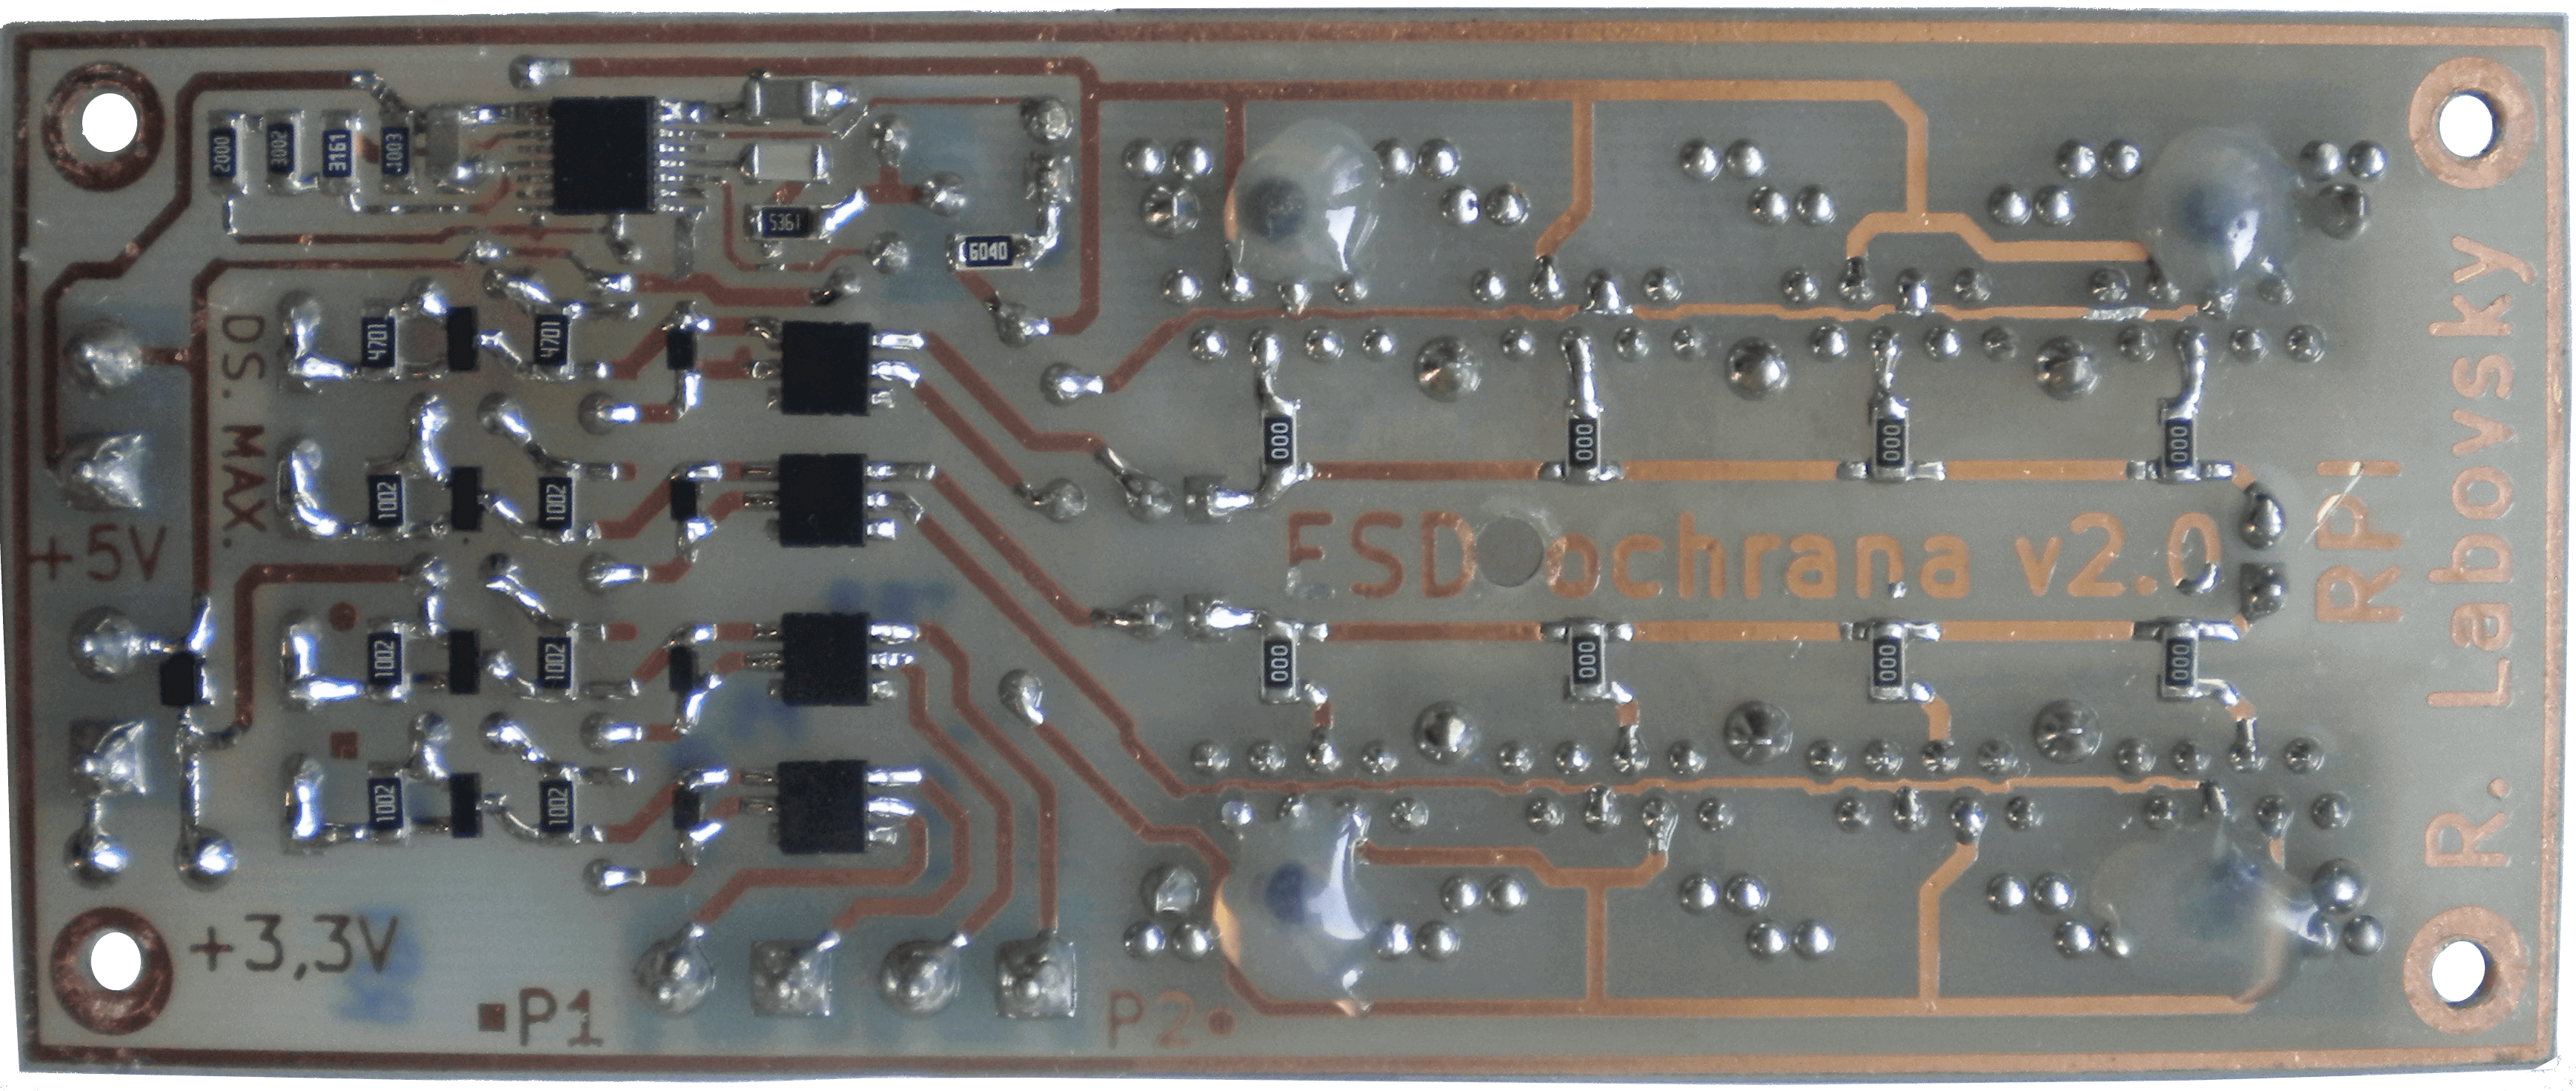
\includegraphics[width=\textwidth]{images/dps-rpi-1-wire-termostaty-ochrany-spodek.png}
    \caption[Spodní část DPS pro ochranu vstupů/výstupů pro Raspberry Pi.]{Spodní část DPS pro ochranu vstupů/výstupů pro Raspberry Pi.}
    \label{fig:dps-rpi-1-wire-termostaty-ochrany-spodek}
\end{figure}

\begin{figure}[H]
    \centering
    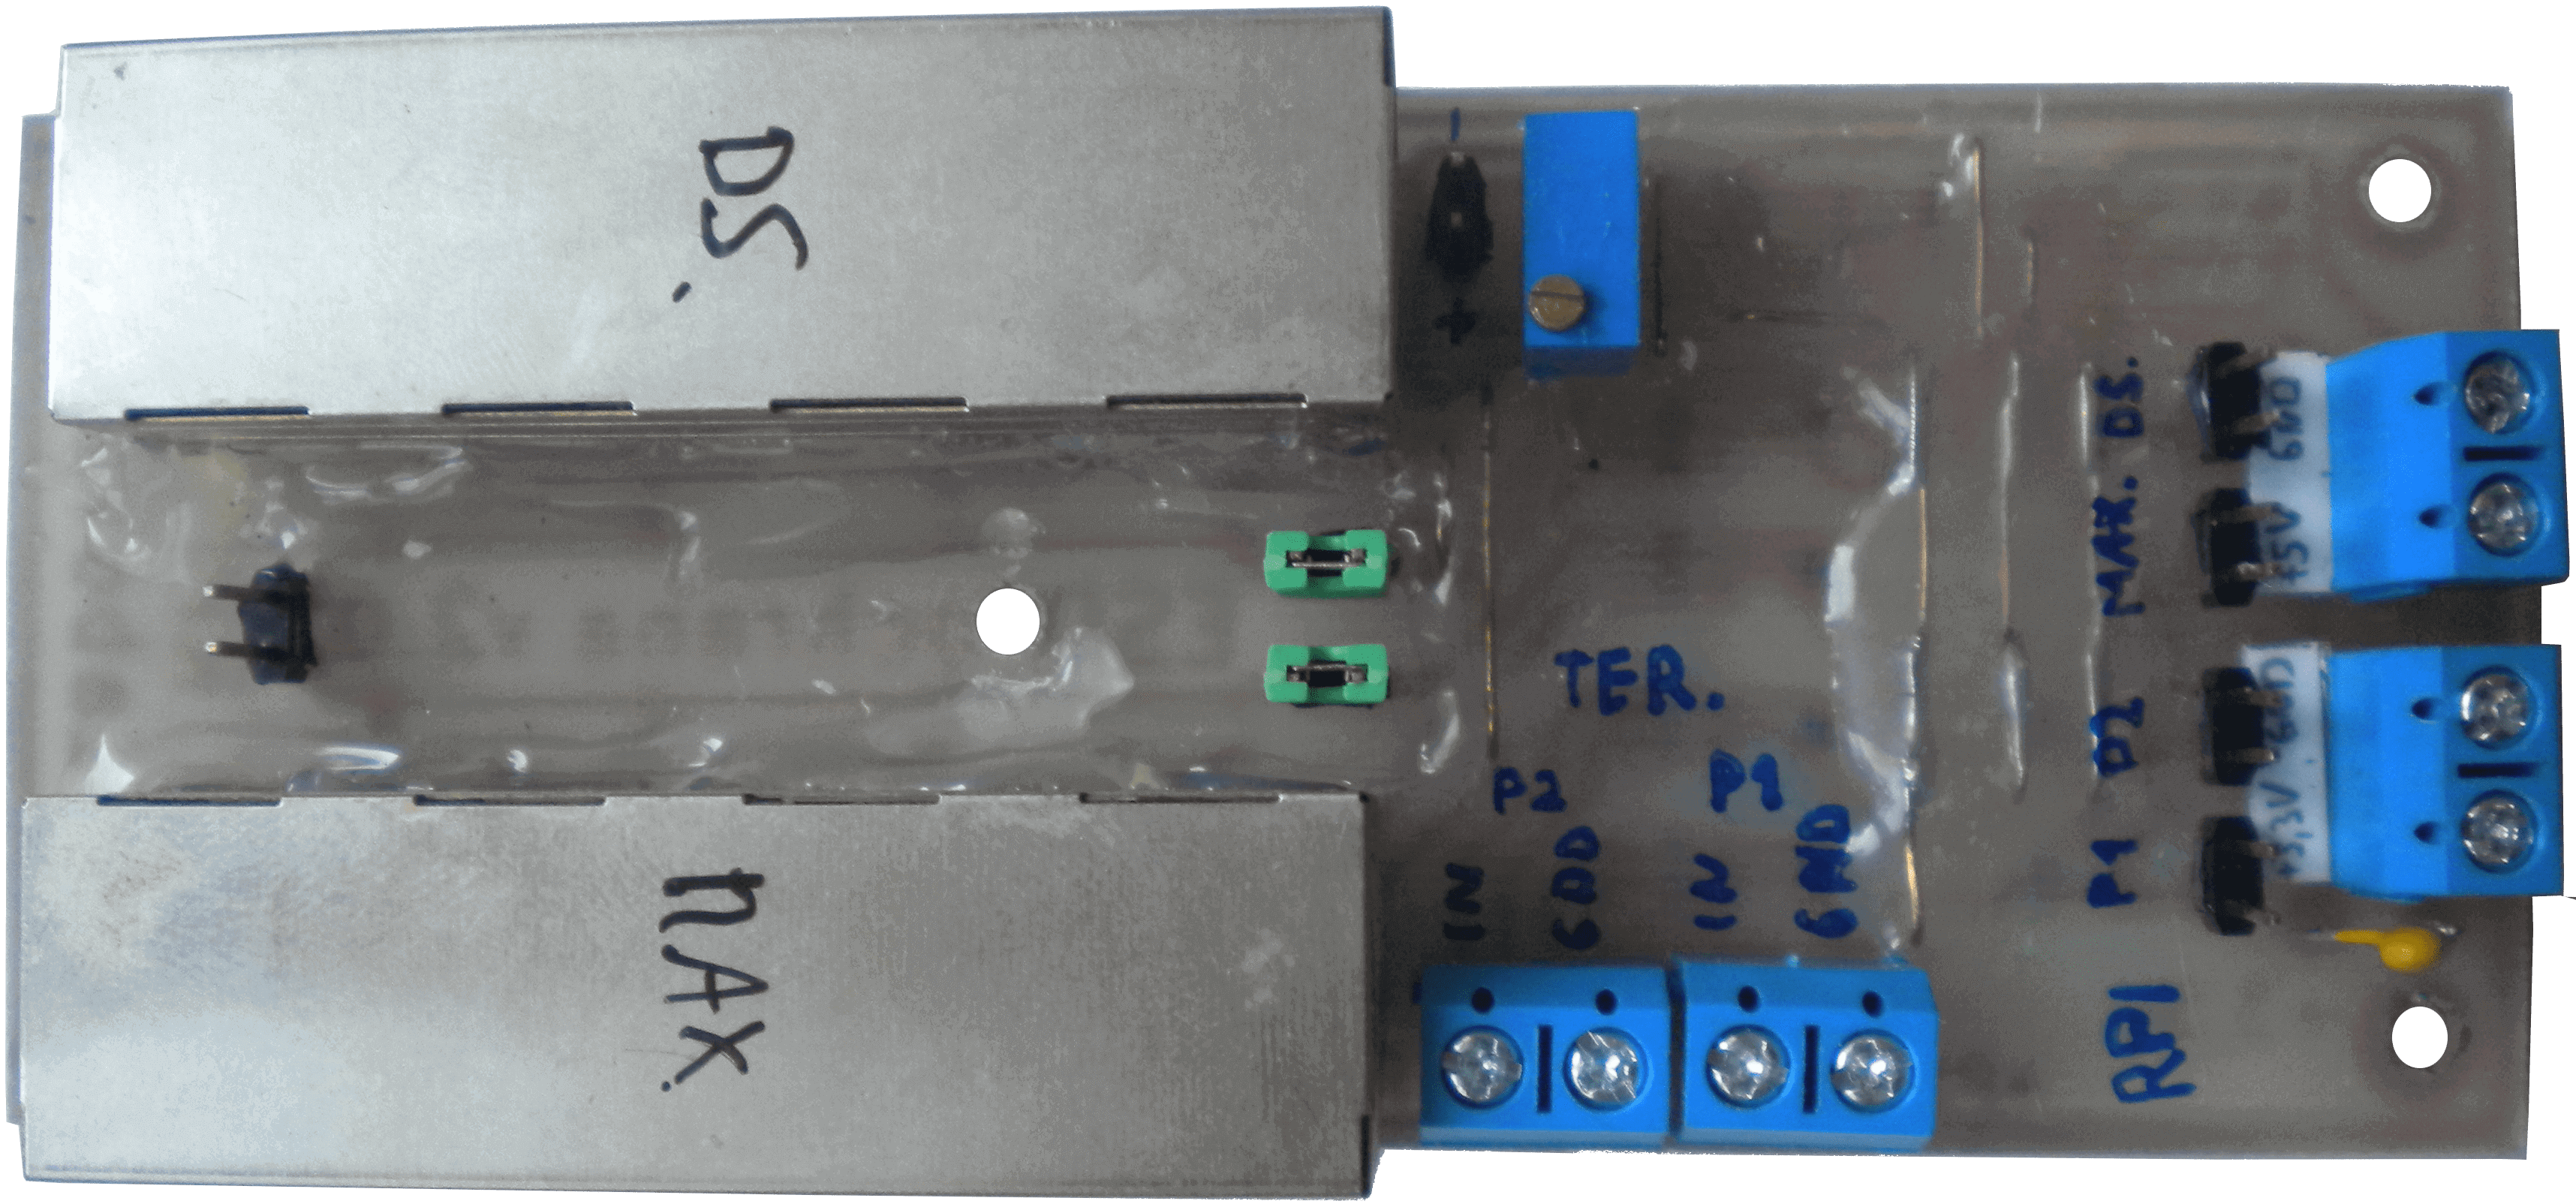
\includegraphics[width=\textwidth]{images/dps-rpi-1-wire-termostaty-ochrany-vrsek.png}
    \caption[Vrchní část DPS pro ochranu vstupů/výstupů pro Raspberry Pi.]{Vrchní část DPS pro ochranu vstupů/výstupů pro Raspberry Pi.}
    \label{fig:dps-rpi-1-wire-termostaty-ochrany-vrsek}
\end{figure}

\section{DPS u krbů}
Navržená DPS se skládá z části elektronické pojistky TPS2600, zapojení je obdobné jako v \ref{napajeni-1-wire-sbernice}, navíc je na vstupu připojena transilová dioda (ESD9L5.0ST5G). Napěťové meze jsou nastaveny stejně, tedy minimální napětí je 4,75 V, maximální 5,25 V, proud je omezen na maximální hodnotu 100 mA. Dále je zde přivedena 1-Wire sběrnice přes konektor RJ45 s obdobnými ochranami jako v \ref{sec:datova-cast-1-wire-sbernice}, včetně stejných ochran pro napájení, pro připojení MAX31850K přes svorkovnici. V neposlední řadě je zde vstupy pro ovládání třech LED pro signalizaci (obrázek \ref{fig:ochrana-krby-lcd-teplotni-senzor}), jak je moc naakumulovaná zásobník otopné vody, modrá led signalizuje stav horní části zásobníku, oranžová LED je pro střední část, červená je pro signalizaci spodní části. Vstupní část je chráněná přes DS9503 a transilovou diodou (ESD9L5.0ST5G). Sepnutí LED je přes tranzistor BSS138P,215. Obdobně jsou řešené i oranžová a modrá LED.

\begin{figure}[H]
    \centering
    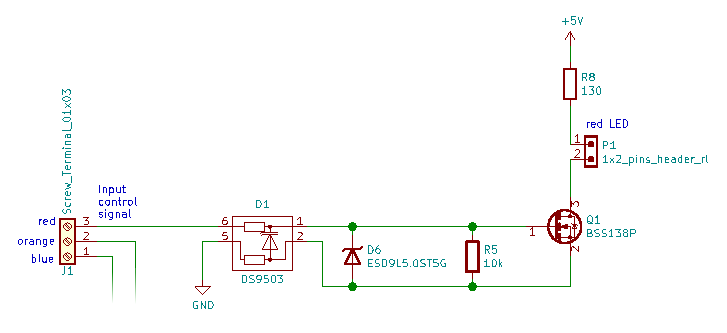
\includegraphics[width=\textwidth]{images/svg/kicad/ochrana-krby-lcd-teplotni-senzor.eps}
    \caption[Zapojení pro ovládání signalizační červené LED.]{Zapojení pro ovládání signalizační červené LED.}
    \label{fig:ochrana-krby-lcd-teplotni-senzor}
\end{figure}

\subsection{I$^2$C sběrnice}
Sběrnice I$^2$C je realizovaná pomocí zakoupeného modulu s obvodem PA9615 do firmy  NXP Semiconductors. Vstupní signál SCL a SDA je veden přímo z centrální jednotky na vstupu obovodu PA9615, napájení je s 3,3 V logikou. Výstup z PCA9615 je pomocí diferenciální vedení, pro každý signál SCL a SDA jsou použity dva vodiče. Napájení na této straně je pomocí 5 V. Sběrnice je realizovaná pomocí UTP cat5E, výstup z modulu je realizován pomocí konektoru RJ45, modulu je na obrázku \ref{fig:pca9615-i2c-sbernice}. Jeden modul se nalézá na straně centrální jednotky a pak na straně krbů. Napájení pomocí 5 V je realizováno pomocí samostatných kabelů, není tedy součástí UTP kabelu. Z důvodu omezení kabeláže je sběrnice realizována v jednom UTP kabelu s 1-Wire sběrnicí, tedy přesněji jsou využity volné vodiče s číslem 1,2 pro SCL a 7, 8 pro SDA. Zařízení lze zapojovat jak na straně před PCA9615, tak i na diferenciální straně, je však výhodné připojené uzly udržet co v nejkratší vzdálenosti kvůli degradování výkonu.

\begin{figure}[H]
    \centering
    \def\svgwidth{\columnwidth}
    \input{images/svg/pca9615-i2c-sbernice.pdf_tex}
    \caption{Blokové schéma zapojení obvodu PCA9615 s impedančním zakončením sběrnice a možnostmi napojení uzlů. Upraveno z \cite{pca9615-schema-zapojeni}.}
    \label{fig:pca9615-i2c-sbernice}
\end{figure}

\begin{figure}[H]
    \centering
    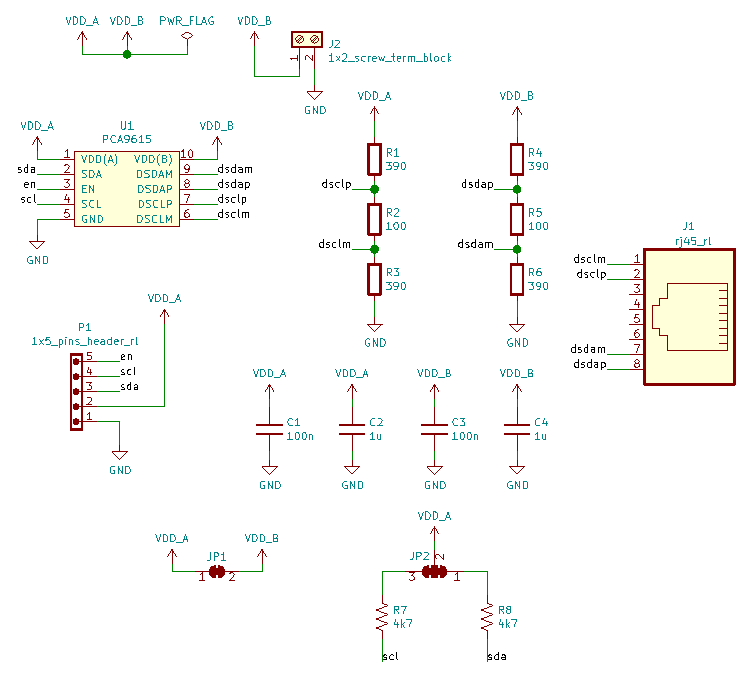
\includegraphics[width=\textwidth]{images/svg/kicad/pca9615-i2c-sbernice.eps}
    \caption{Zapojení PCA9615 v modulu. Upraveno z \cite{pca9615-schema-zapojeni}.}
    \label{fig:pca9615-i2c-sbernice}
\end{figure}

Výhodou PCA9615 je automatický výběr směru komunikace, není potřeba externího ovládání pro ovládání směru komunikace. Komunikace je možná až do rychlosti 1 MHz (přibližně pro 3 m), se zvýšenou délkou je však nutné rychlost snížit. Komunikace využívá standardního protokolu I$^2$C. ESD ochrana, v případě naindukování přepětí po cestě. Nezávislost napájení, je možné napájet koncová zařízení z jiného zdroje než Master. V neposlední řadě se jedná o jednoduché řešení bez nutných další zařízení na straně Slave, stačí pouze zapojit koncové zařízení s podporou I$^2$C.

\begin{figure}[H]
    \centering
    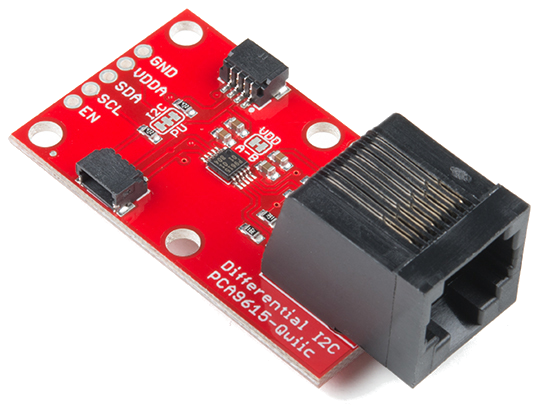
\includegraphics[width=0.6\textwidth]{images/pca9615-i2c-sbernice.png}
    \caption[Modul s obvodem PCA9615.]{Modul s obvodem PCA9615 \cite{pca9615-i2c-modul}.}
    \label{fig:pca9615-i2c-sbernice}
\end{figure}

\subsection{}
Teplotní senzory připojené na kouřovody krbů realizované pomocí termočlánku z \ref{sec:teplotni-senzory-pro-krby} jsou připojené k zesilovači napětí generované termočlánkem, hodnota napětí je následně převedena do digitální podoby včetně teplotní kompenzace studeného konce termočlánku a tato hodnota je posílaná po 1-Wier sběrnici.

\begin{figure}[H]
    \centering
    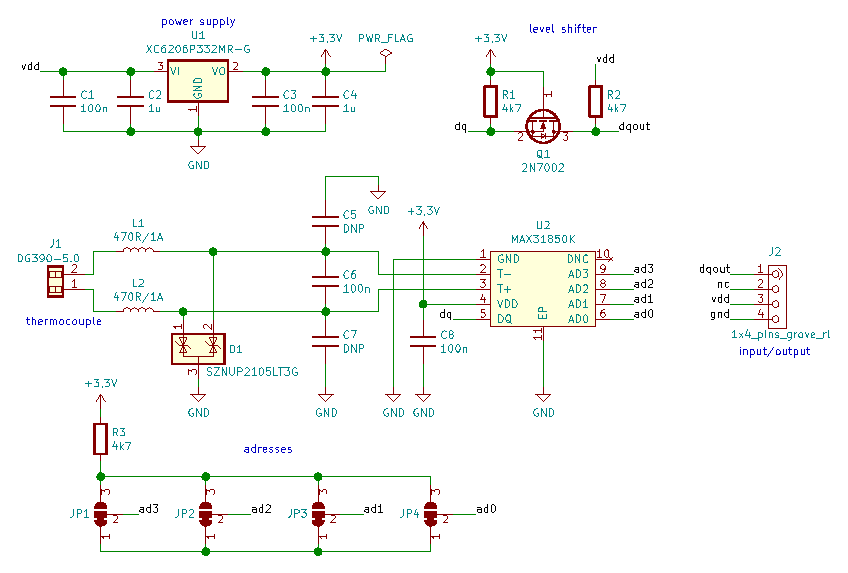
\includegraphics[width=\textwidth]{images/svg/kicad/max31850k-1-wire-prevodnik-termoclanku.eps}
    \caption{. Upraveno z \cite{}.}
    \label{fig:max31850k-1-wire-prevodnik-termoclanku}
\end{figure}

\begin{figure}[H]
    \centering
    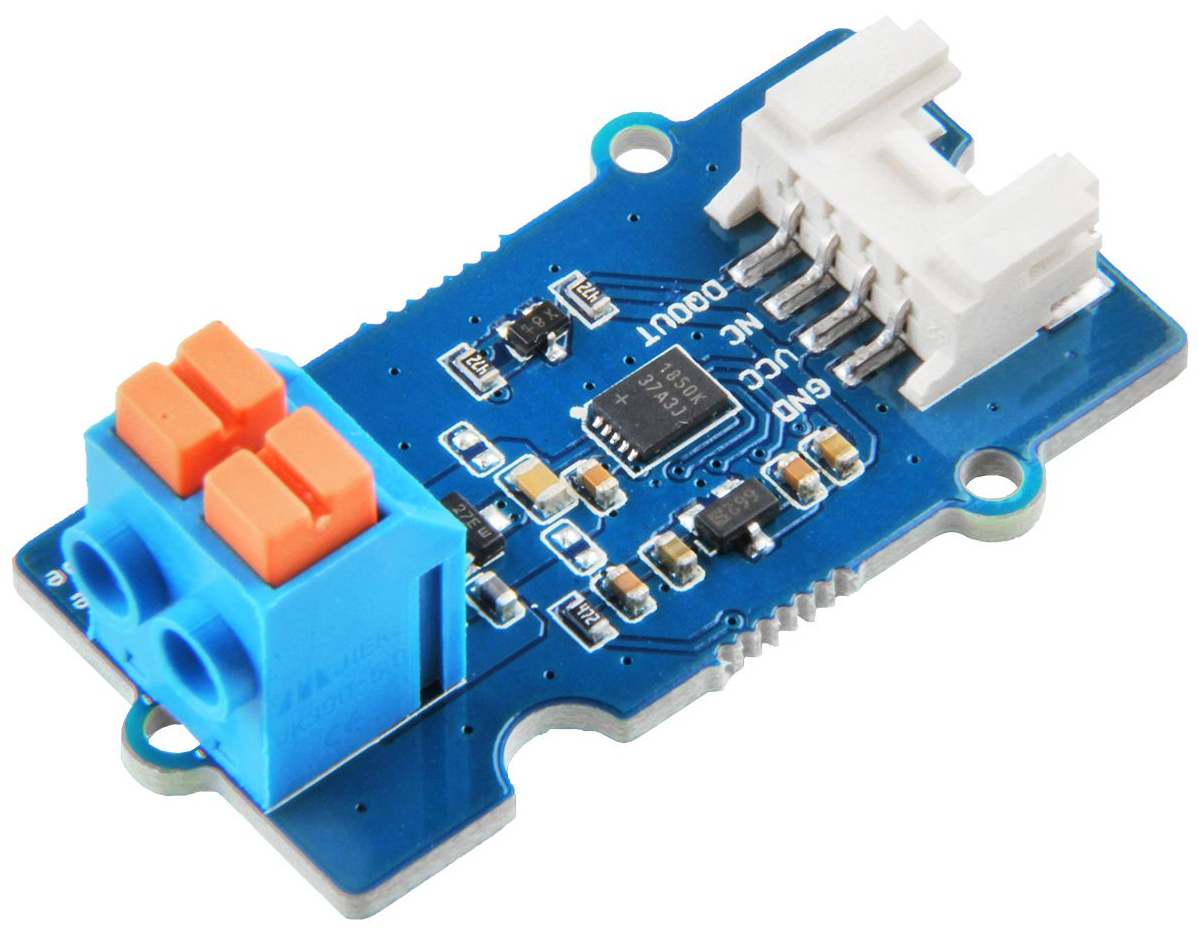
\includegraphics[width=0.6\textwidth]{images/max31850k-1-wire-prevodnik-termoclanku.png}
    \caption[]{}
    \label{fig:max31850k-1-wire-prevodnik-termoclanku}
\end{figure}

